\documentclass[11pt]{article}
\usepackage[preprint]{acl}
\usepackage[T1]{fontenc}
\usepackage[utf8]{inputenc}
\usepackage{times,latexsym,amsmath,amssymb,booktabs,graphicx}
\usepackage{microtype}
\title{When Is Changed Communication Credit Worth Checking?\\A Costed Study of Small Language Model Collaboration}
\author{Research draft for author review}
\begin{document}
\maketitle
\begin{abstract}
Deleting an upstream communication edge can change the value of a downstream edge. Whether a system can profitably detect that change before serving new requests is a separate empirical question. We study both questions with paired graph interventions, matched acquisition budgets and explicit charges for initialization, discarded probes and service. In a previously collected 512-question service cohort, an active policy gains 0.00093 utility over random checks and loses 0.00408 to stale credit. A subsequent coding pilot yields 16 successful graph decisions across 48 question--seed pairs, compared with 23 for early-stopped independent sampling. On two multi-hop QA development cohorts, a selector with access to future outcomes attains sizeable gains. A feasible historical-panel estimator misses the matched-budget criterion in all six task--acquisition-seed combinations. We identify configurations with too little decision opportunity and configurations with measurable opportunity that our estimates fail to capture. These results bound the claims of the tested methods and provide reproducible controls for studying graph-conditioned revalidation.
\end{abstract}

\section{Introduction}
An edge that feeds a useful intermediate answer into a final reader might become redundant when another path begins carrying the same evidence. Conversely, an inexpensive deletion can become destructive after an upstream message disappears. Monitoring every edge by rerunning every graph is expensive. The scientific question is whether past interventions help select a small number of new checks that improve subsequent service decisions.

Previous work has learned sparse communication graphs \citep{agentprune}, dynamically eliminated redundant agents \citep{agentdropout}, and tested the cost and accuracy of debate against simpler alternatives \citep{smit}. These studies motivate strong graph and single-model controls. Our intervention concerns the continued applicability of historical counterfactual feedback after the graph changes. We evaluate the conditions that would make paying for a fresh measurement worthwhile. We find no validated improvement from the tested paid methods. This motivates reporting the intervention effect, the possible decision gain and the realized net benefit separately.

\section{Estimation and evaluation}
For a question $x$, graph $g$ and fixed coupled random state $z$, we measure edge credit as
\begin{equation}
 c_e(x,g,z)=R(x,g,z)-R(x,g\setminus e,z).
\end{equation}
Here $R$ is answer correctness under the declared task metric. A change in $c_e$ can be real even when the preferred action remains the same. A policy first receives an initialization set, pays for selected graph interventions, then chooses actions for service questions. In the QA experiments its utility is
\begin{equation}
 U=\overline R-5\!\times\!10^{-6}(T_I+T_C+T_S)/n_S,
\end{equation}
where $T_I,T_C,T_S$ count inputs and outputs for initialization, checking and service. The coding pilot additionally charges visible program execution as specified in its contract. GPU residence is reported separately. A token price expresses the study's chosen trade-off. It does not measure a vendor price or normalize FLOPs across model families.

For any fixed menu of legal actions, an evaluator can give a selector future outcomes at zero cost. Its utility bounds policies with that menu and information partition when charged costs are nonnegative. The comparator, action set and level of sharing matter. A per-question oracle cannot establish that a single deployment edit works across questions. To distinguish the two, our final experiment restricts one action to each external graph-change type in each service fold.

\section{Design and provenance}
\paragraph{Original prediction and maintenance studies.} The initial value-prediction experiment used 400 questions split into 200 training, 80 tuning and 120 held-out questions. Of 2,880 held-out question--coordinate pairs, 2,187 had zero measured credit on all five seeds. The common noise-adjusted squared risks were 0.001417, 0.001541 and 0.002196 for the three registered predictors. Always predicting zero gave 0.001354. Shrinkage is a strong comparator here. In the later fifth formal experiment, 640 HotpotQA training questions were assigned to initialization, checking and service roles under a separate contract. Five generation seeds shared the same questions. The service set contained 512 questions. Feedback policies used a common predictor and exact terminal-ancestor execution. Each condition paid for all of its active requests.

\paragraph{Further formal pilots.} We tested evidence-indexed communication, raw-evidence-preserving annotations on HotpotQA and 2Wiki, long-document reading on Qasper, and code generation on APPS. HotpotQA is a multi-document QA dataset \citep{hotpot}. The annotation transfer used each task's scoring rule and different questions. The long-document pilot contained 16 papers and two sampling seeds. The independent confirmation cohorts associated with failed admission gates stayed sealed. We keep all earlier gates and negative outcomes.

\paragraph{APPS pilot.} We used 16 training questions with a qualified function interface, three generation seeds and ten original conditions per question. Code was generated by Qwen2.5-3B-Instruct and Qwen2.5-Coder-7B-Instruct under fixed prompts. Visible examples supported workflow decisions. Success required passing all held-back program cases for that problem. An interrupted six-question segment and a resumed ten-question segment contributed to the final matrix. We reconstructed both segments and ran a local isolated evaluator before releasing any pilot hidden-case result. The 128 independent confirmation problems remained sealed.

\paragraph{Historical-panel replay.} We used archived interventions on 96 HotpotQA and 96 2Wiki development questions. For each question we had two source-message realizations, four terminal seeds and eight message subsets. An exogenous removal left two remaining incoming edges. An action could retain both, remove either or use the no-message reader. Four question-disjoint folds rotated service. Within each fold we chose four historical panel questions per shock type from outside service. All policies that initialize paid for the original graph, its three single deletions and the no-message output on these twelve questions, with request-level cache sharing. Exact duplicates were credited equally to all policies.

The paid policies revisited one historical question per shock type, three in total. The candidate estimated each current action from its old observed reward plus the observed change in base-graph reward. A prior identical terminal request gave the exact old reward for that request. It sampled historical questions preferentially when the graph change or old deletions altered their rewards, retaining positive selection probability for every item. It corrected the panel estimate with the selected question's inverse-probability-weighted residual. Uniform, periodic and uncertainty selection shared the estimator. An ablation dropped the residual correction and used the selected question directly. Additional controls reused old decisions, used the initial estimate without rechecking, or deployed a fixed edit or single reader without initialization. The maximum budget was 800,000 tokens per 24 service questions. Unused budget incurred no charge. We tracked three acquisition seeds, with the same previously recorded generations for every method. The two-task gate required a gain of at least 0.005 over the best matched control and nonnegative utility against the best cheap control for every acquisition seed.

\section{Results}
\paragraph{The fixed maintenance policy on HotpotQA.} The fifth formal nominee and random checking each achieved 60.51\% exact match. Their full utilities were 0.56722 and 0.56628. The stale-credit control reached 0.57129. A free structural control that removed the other direct edge reached 0.58461. We subsequently tested whether that last result was attributable to the shock identity. After matching the nominal affected side in a no-shock placebo, the incremental utility interaction was 0.00225. It was negative for U shocks and positive for V shocks. The free rule's gain over the best fixed-identity or keep strategy was 0.00005. The higher point estimate alone did not identify a portable structural rule.

\paragraph{Graph quality and sparse coding credit.} In the two annotation studies, 39 HotpotQA and 32 2Wiki question groups showed a credit change. The candidate's exact match fell below direct Qwen by 5.73 and 20.31 percentage points. In Qasper the graph's F1 was 0.3941 versus 0.3793 for dense retrieval, yet token utility was 0.3021 versus 0.3544. In APPS, Table~\ref{tab:apps} shows that a more expensive graph also solved fewer instances than early-stopped sampling. Relative to that baseline the graph corrected four decisions and damaged eleven, with 33 ties. Across seeds its utility differences were $+0.0430$, $-0.2074$ and $-0.3319$. One of 96 current edge observations had nonzero hidden credit. This one event is insufficient for calibrating visible feedback reliability.
\begin{table}[t]\centering\small
\setlength{\tabcolsep}{4pt}\begin{tabular}{@{}lrrr@{}}\toprule Policy & Solved/48 & Utility & Tokens\\\midrule
Graph selection &16&.3089&4,887\\ Direct 7B &20&.4139&544\\ Three samples, early stop &23&.4743&977\\ Three repairs &22&.4518&1,307\\ Reuse requested history &17&.3097&8,887\\\bottomrule\end{tabular}
\caption{APPS pilot on 16 questions and three shared generation seeds. Tokens are means per question--seed decision.}\label{tab:apps}\end{table}
\begin{figure*}[t]\centering
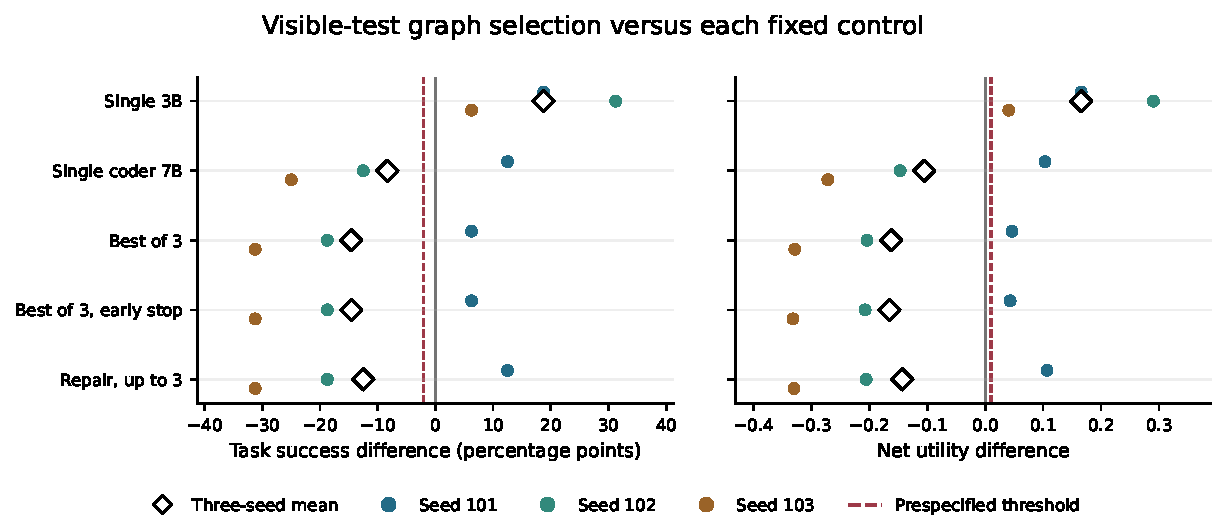
\includegraphics[width=.80\textwidth]{../../reports/cycle3_20261116/formal10_function/PILOT_COMPARISONS.pdf}
\caption{Coding-pilot performance and paired comparisons under the frozen cost rule. Each of the 16 problems contributes three shared model seeds. The accompanying report contains the counts of corrections and harms.}\label{fig:pilot}\end{figure*}

\paragraph{From future-label selection to paid selection.} On the archived QA tasks, even a selector restricted to one action per shock in each evaluation fold can perform well when it knows the outcomes. Its utility gains over the strongest of the four frozen cheap controls were 0.09523 on HotpotQA and 0.05095 on 2Wiki. The gains were positive on each fold against the old shock-conditioned policy. This is an optimistic, fold-specific opportunity bound. Approximately eight service examples per shock type can make future-label selection look especially attractive. Training on current-graph labels from other questions yielded utility 0.5470 on HotpotQA and 0.6332 on 2Wiki, illustrating how much can change when the labels move across questions.

Under actual acquisition, Table~\ref{tab:paid} shows no seed meeting the matched-budget margin. Every comparison with the strongest cheap control was negative. Two panels may contain different mixes of pivotal questions even when both have the same shock identity. Our design cannot isolate sampling variance, error in the transferred prior and incomplete task features as competing explanations.
\begin{table}[t]\centering\small
\begin{tabular}{lrrr}\toprule Task & Seed & Matched $\Delta U$ & Cheap $\Delta U$\\\midrule
HotpotQA &17&$-.01775$&$-.07389$\\&31&$-.02904$&$-.05556$\\&47&$-.03086$&$-.07130$\\\addlinespace
2Wiki &17&$-.02268$&$-.05183$\\&31&$.00000$&$-.07196$\\&47&$-.01106$&$-.06906$\\\bottomrule\end{tabular}
\caption{Candidate minus best comparator in each prespecified class. Utilities include all stages. Seeds change acquisition, not the service questions.}\label{tab:paid}\end{table}

\section{Further mechanism checks}
TimeQA training annotations link answer character offsets to an evidence passage. We selected one pair of non-overlapping temporal questions within the same article and relation, using only input information. Of 64 selected articles, 46 yielded a verifiable support paragraph for both queries. Modifying the retrieval graph at fixed question time changed credit in nine articles. Only five articles offered two different current selections, and perfect rechecking could repair one error. Every equal-budget policy covered those five and reached 23 correct selections. This experiment tested paragraph retrieval on retrospective articles. It did not observe a changing Wikipedia snapshot.

A second check replayed six small models on the 1,267 public WinoGrande validation questions in LLMRouterBench. We grouped near duplicates and adjacent released items into 488 groups across three folds. Each deployment selected a fixed subset of model answers before receiving service labels. Direct Qwen3-8B obtained 82.79\% accuracy. Even choosing the utility-maximizing fixed graph per service fold with its labels gave 81.85\% accuracy and 0.80892 utility, compared with 0.82219 for direct Qwen. These are upstream cached answers with deterministic terminal aggregation. They do not measure adaptive message generation. Across the two checks, one setting lacked any budget scarcity after trivial equal-output cases were removed, and another had a graph menu below a cheap comparator. Those mechanisms differ from the positive future-label opportunity in multi-hop QA.

\section{Limitations and conclusion}
The experiments involve selected tasks, finite edit menus, short service horizons, fixed model pools and benchmark labels as a feedback oracle. Repeated seeds share questions. Several later analyses reuse exposed development data and cannot provide independent confirmation of a learned policy. We did not execute an external graph-pruning or debate implementation under identical resource and input constraints. Cost conclusions depend on the declared token trade-off. Unknown costs, including two interrupted requests' tokens, were left unknown. No population confidence interval or bootstrap was computed under the protocol. The results support decisions about these configurations. They do not establish impossibility or a state-of-the-art ranking.

We found direct evidence for graph-dependent credit and for useful choices available to a future-label oracle. Neither was sufficient to justify the tested feedback policies. A study reporting a revalidation benefit should show that the current edit menu can beat simple deployment, that the acquisition rule identifies errors prospectively, and that the gain survives the cost of discovering them.

\paragraph{Dataset provenance.} We use the authors' scoring conventions for 2Wiki \citep{twowiki} and Qasper \citep{qasper}, and training cases from APPS \citep{apps}. The temporal reading material comes from TimeQA \citep{timeqa}. The WinoGrande validation task \citep{wino} was obtained through the \href{https://github.com/ynulihao/LLMRouterBench}{LLMRouterBench author release}. Validation cache exposure precludes independent confirmation on those records.

\section*{Reproducibility and responsible use}
The code, contracts, per-fold summaries and cost reports are organized by experiment in the companion MAB2 repository. Source datasets retain their authors' terms. The public artifacts omit question-level material and model weights. Replaying the private scored matrices requires authorized local access. We used AI research and writing assistance, including the scientific-writing and peer-review procedures described by \citet{skills}. This is an author-side draft. No independent human review or submission has occurred.

\begin{thebibliography}{10}
\bibitem[Ho et~al.(2020)]{twowiki} Xanh Ho et~al. 2020. \href{https://aclanthology.org/2020.coling-main.580/}{Constructing A Multi-hop QA Dataset for Comprehensive Evaluation of Reasoning Steps}. In COLING.
\bibitem[Dasigi et~al.(2021)]{qasper} Pradeep Dasigi et~al. 2021. \href{https://aclanthology.org/2021.naacl-main.365/}{A Dataset of Information-Seeking Questions and Answers Anchored in Research Papers}. In NAACL.
\bibitem[Hendrycks et~al.(2021)]{apps} Dan Hendrycks et~al. 2021. \href{https://arxiv.org/abs/2105.09938}{Measuring Coding Challenge Competence With APPS}. In NeurIPS Datasets and Benchmarks.
\bibitem[Chen et~al.(2021)]{timeqa} Wenhu Chen et~al. 2021. \href{https://arxiv.org/abs/2108.06314}{A Dataset for Answering Time-Sensitive Questions}. In NeurIPS Datasets and Benchmarks.
\bibitem[Sakaguchi et~al.(2020)]{wino} Keisuke Sakaguchi et~al. 2020. \href{https://arxiv.org/abs/1907.10641}{WinoGrande: An Adversarial Winograd Schema Challenge at Scale}. In AAAI.
\bibitem[Yang et~al.(2018)]{hotpot} Zhilin Yang et~al. 2018. \href{https://aclanthology.org/D18-1259/}{HotpotQA: A Dataset for Diverse, Explainable Multi-hop Question Answering}. In EMNLP.
\bibitem[Zhang et~al.(2025)]{agentprune} Guibin Zhang et~al. 2025. \href{https://arxiv.org/abs/2410.02506}{Cut the Crap: An Economical Communication Pipeline for LLM-based Multi-Agent Systems}. In ICLR.
\bibitem[Wang et~al.(2025)]{agentdropout} Zhexuan Wang et~al. 2025. \href{https://aclanthology.org/2025.acl-long.1170/}{AgentDropout: Dynamic Agent Elimination for Token-Efficient and High-Performance LLM-Based Multi-Agent Collaboration}. In ACL.
\bibitem[Smit et~al.(2024)]{smit} Andries Petrus Smit et~al. 2024. \href{https://proceedings.mlr.press/v235/smit24a.html}{Should we be going MAD? A Look at Multi-Agent Debate Strategies for LLMs}. In ICML.
\bibitem[Kassis et~al.(2026)]{skills} Timothy Kassis, Vinayak Agarwal, Yuhuan He, Darshil Patel, and Aubrey M. Brueckner. 2026. \href{https://arxiv.org/abs/2609.00065}{Scientific Agent Skills: A Library of Procedural Knowledge for Research Agents}. arXiv:2609.00065.
\end{thebibliography}
\appendix
\section{Reproduction map and cohort boundaries}
The earlier five-route paper and its supplementary tables are in \texttt{paper/closure\_study\_v1}. Formal experiments 6--10 each have a separate frozen report. The APPS audit reconciles 480 original condition cells, 369 distinct programs within questions, 1,797 hidden executions, and 7,884 scalar consistency checks. Two interruption-time returns lack token counts. The coding route consumed 3.08834 GPU residence hours including qualification. Project use closed at 93.37976 out of 160 GPU hours. Later CPU replays used no new GPU inference.

The source audit D28 found prior ancestor prompts for all 100 candidate EvoEval lineage families. Those families cannot serve as independent confirmation for this project. D29--D30 used only the exposed APPS pilot. D31--D32 used training files and D33 used a public validation cache. D34 used the already-exposed fifth formal service results. D35--D36 used the D16 development cohorts. Service labels in D36 were used only after policy actions were determined in each fold. An independent scalar implementation reconstructed 288 policy--fold records and passed 4,346 comparisons of actions, paired outcomes and costs. These checks establish consistency of the recorded development results. Human reproduction, generalization to new traffic and a complete evaluation of a novel positive method remain open.
\end{document}
